\section{Implementation}\label{sec:web_ping_impl}

To collect data, the site dynamically inserts \html \texttt{img} tags pointing to a number of small resources, each owned by one of the top 50 sites in the \us. Before \texttt{img} tag insertion, the site records the current time, then records the time upon completion of loading; this method is shown in \cref{code:web_ping_code}. Once resources from all 50 sites have been loaded, the client packages the data into a \json object and sends it via web socket to the server, which stores the data in a MongoDB database. 

\begin{code}[h]
    \centering
    \small
    \begin{minted}{JavaScript}
function ping(url) {
  return new Promise(function (resolve, reject) {
    const start = (new Date()).getTime();
    const response = function () {
      let delta = ((new Date()).getTime() - start);
      resolve(delta);
    };
    request_image(url).then(response).catch(reason => reject(reason));
  });
}
    \end{minted}
    \caption{JavaScript "ping" function}
    \label{code:web_ping_code}
\end{code}

\subsection{Front end}

For the website itself we used the JavaScript Library \texttt{D3.js} ("D3") to draw the maps. D3 is a library specifically designed for data visualization of large data-sets. To draw the states themselves, D3 loads a \json file containing a definition of the map and renders it as an \svg image on the screen. To draw points for each city, collected data is passed into D3, following the format \texttt{\small [\{favicon: "facebook.com", avg\_rtt: 1.1, city: "Boston", latitude: 0.0, longitude: 0.0\}]}. D3 then converts the longitude and latitude to coordinates on the screen and uses a a color gradient based on the \rtt to determine the color of the dot. An example of such a map is displayed in \cref{fig:siteping_city}.

Initially, we used the absolute minimum and maximum values of the data to determine the limits of the gradient, but we found that color gradients would often be skewed towards outliers. To solve this problem, we switched to using the minimum and maximum of the inter-quartile range of the data set for the color gradient. All of the points outside this range are displayed as pure red or pure white. This eliminates outlier effects while staying fast enough to be performed on the server or in the browser, as opposed to slower methods like z-score filtering.

\begin{figure}[h]
    \centering
    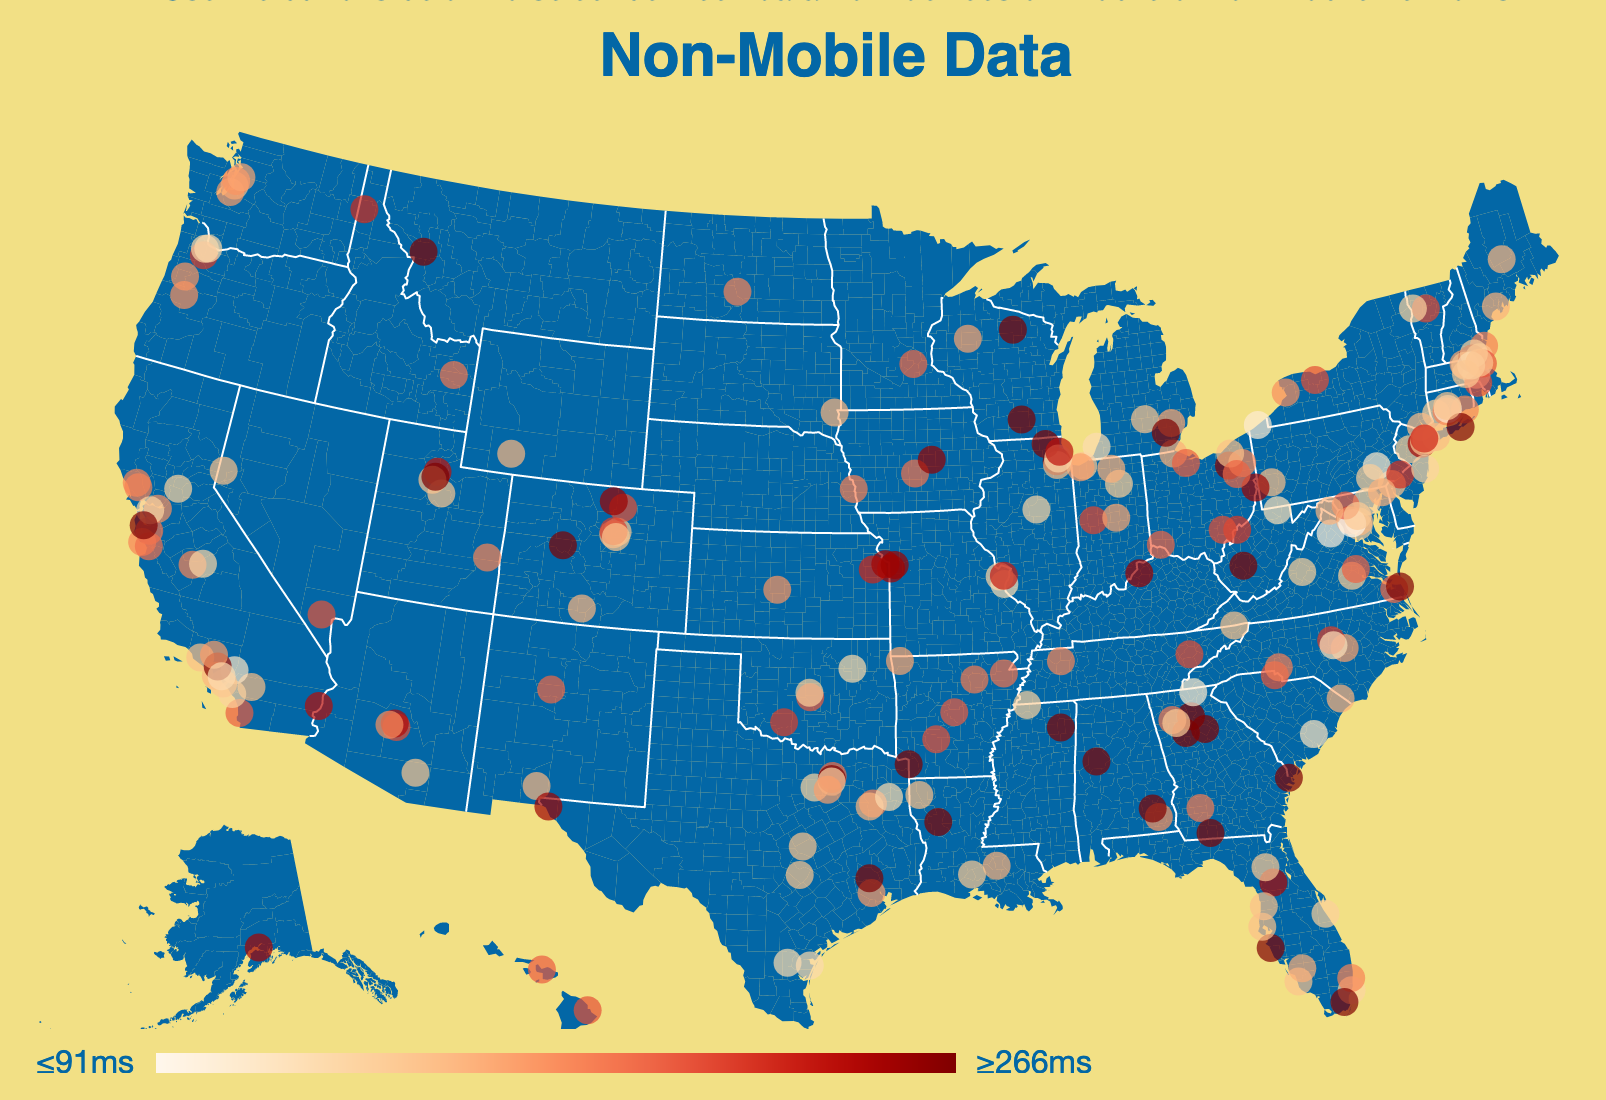
\includegraphics{siteping/cityview.png}
    \caption{Site ping city view}
    \label{fig:siteping_city}
\end{figure}

\subsection{Back end and Database}

When a client sends data to the server, the server uses the MaxMind geolocation database to assign the data a latitude and longitude. All of this information is stored in the database, and additionally is sent via web sockets to all of the other connected clients so the site map can update in real time. For the back-end database, we chose to use MongoDB to host all of our data, which is queried by the server when a client connects. We chose MongoDB because of its simple and free cloud hosting platform (known as Atlas), as well as the ease of integration with NodeJS (our chosen server platform). The backend web server was a NodeJS server hosted on an \aws \ecc instance.

\subsection{Distribution}

We tried multiple ways to distribute the site to people across the \us. To track site usage, we used Google's free web analytics suite, aptly called "Google Analytics." Google Analytics works using an embedded block of JavaScript in the site, gathers information about the user's browser and activity. The script can also read other cookies and metadata to determine where the user came from and how long they remained on the site. Finally, the collected information is encoded into the metadata of a request for a one pixel image \cite{GoogleGoogleOverview}.

\subsubsection{Reddit}

The site was first distributed on Reddit, a popular message board and content aggregation site. We posted in two communities, \href{https://reddit.com/r/dataisbeautiful}{/r/dataisbeautiful} (14.2 million readers) and \href{https://reddit.com/r/samplesize}{/r/samplesize} (121k readers). Unfortunately, posting on Reddit proved unsuccessful and gained us only around 10 views. Since many people sort by popular posts and our post never received much attention, few people saw it.

\subsubsection{Facebook}

One of our most successful methods for distributing the site was through Facebook. Initially, one of our members posted it on his own personal page, after which the site received a few views. Soon afterwards, a family member posted the link into the \wpi parents' Facebook group, resulting 125 views across the \us. Finally, a group member posted the link to four of the \wpi undergraduate Facebook groups, resulting in a further 70 views of the site. We intentionally waited to post to the \wpi undergraduates Facebook group until winter break started, hoping to maximize the geographic diversity. The timeline of visits to the site originating from facebook is displayed in \cref{fig:siteping_facebook_usage}.

\begin{figure}[h]
    \centering
    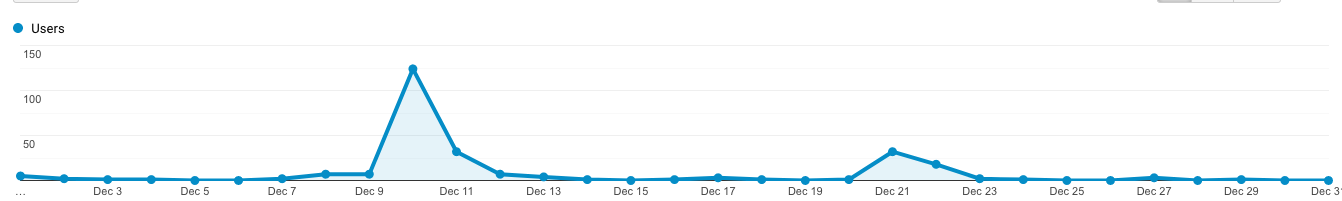
\includegraphics{siteping/usage/facebook-usage.png}
    \caption{Facebook site visit}
    \label{fig:siteping_facebook_usage}
\end{figure}

\subsubsection{Amazon Mechanical Turk}

To reach people in states lacking data, we turned Amazon's "Mechanical Turk" service. Mechanical Turk is a crowd sourcing platform that allows people to pay others ("workers") to complete small online tasks ("HITs"). We paid 1-50 cents for users in states that we had little data for, with higher amounts for sparser states to incentivize workers to complete our HITs. When someone selected our task, they were directed to a special \url on the site ping website. When began data collection and waited for two cycles worth of data, they were given a token which they copied and pasted into Mechanical Turk to ensure that they actually completed the task. The tokens were generated using a JavaScript web token module for NodeJS which the server could verify; only after verification were workers paid. Using Mechanical Turk resulted in an additional 221 visits to the site, bringing the total of covered states up to 47.

\begin{figure}[h]
    \centering
    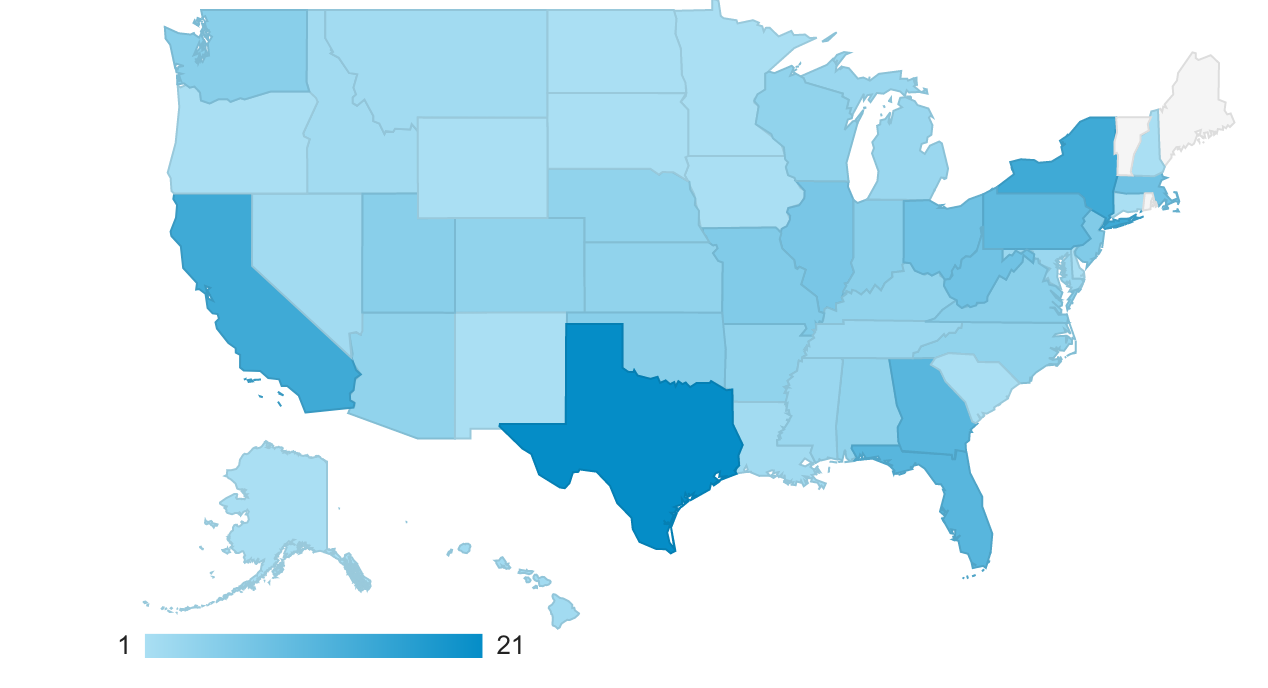
\includegraphics{siteping/usage/mturk-distribution.png}
    \caption{Involvement from Mechanical Turk by state}
    \label{fig:siteping_mturk_distribution}
\end{figure}

% \subsubsection{Email}
